\documentclass{article}
\usepackage{times}
\usepackage{amsmath}
\usepackage{mathptmx}
\usepackage{textcomp}
\usepackage{graphicx}
\usepackage{color}
\usepackage{xspace}
\usepackage[caption=false]{subfig}
\usepackage{multirow}
\usepackage[compact]{titlesec}
\usepackage{float}
\usepackage{epstopdf}
\usepackage{balance}



\setlength{\textwidth}{6.5in}
\setlength{\textheight}{9.50in}
\setlength{\oddsidemargin}{-.19in}
\voffset=-1.0in

\title{CS 690LG Project: Parallel SAT Solving}
\author{Prateek Sharma}



\begin{document}
\maketitle
\section{Introduction}


\section{Project scope}


\section{ManySAT}

\subsection{Experiment Platform}
Experiment setup

\begin{figure}[h]
  \centering
  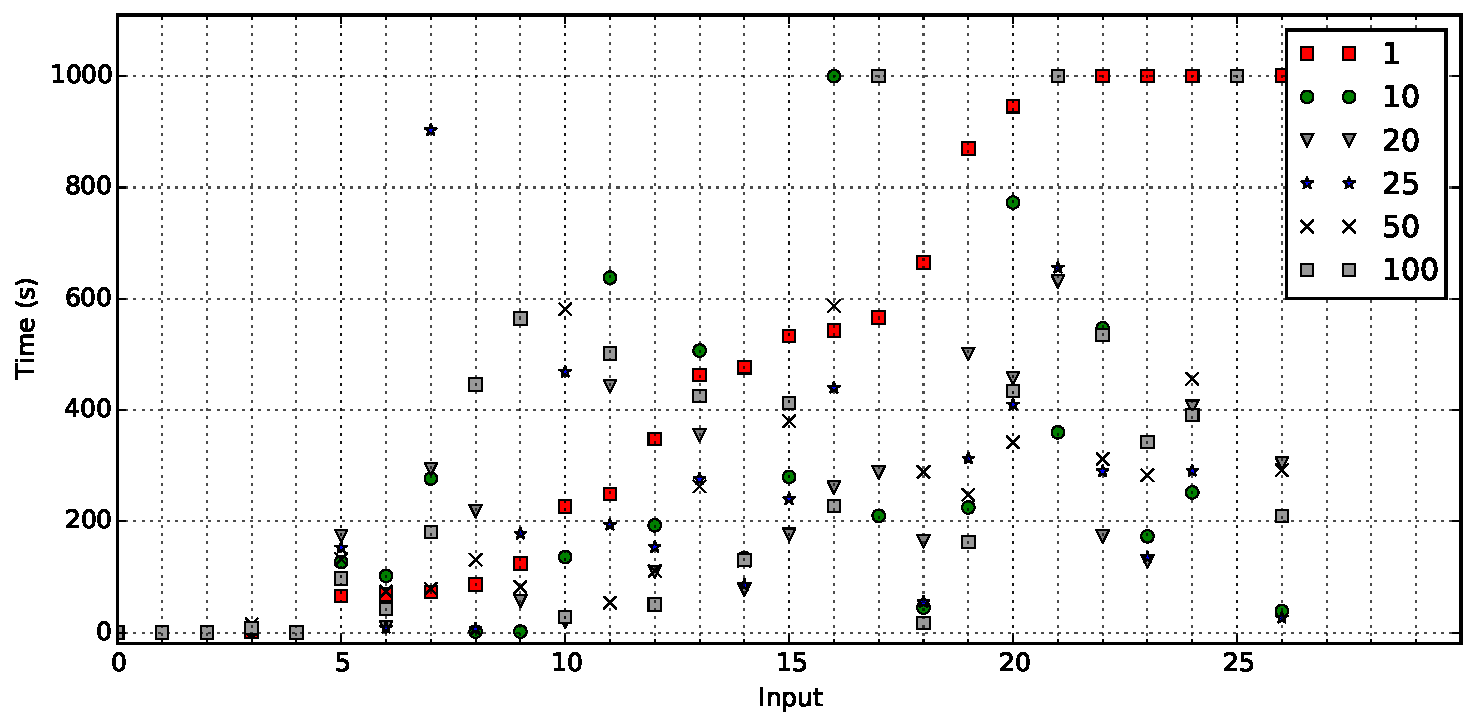
\includegraphics[width=0.8\textwidth]{../figs/scatter_all.pdf}
  \caption{Scatter-plot of running times}
  \label{fig:scatter-1}
\end{figure}

\begin{figure}[h]
  \centering
    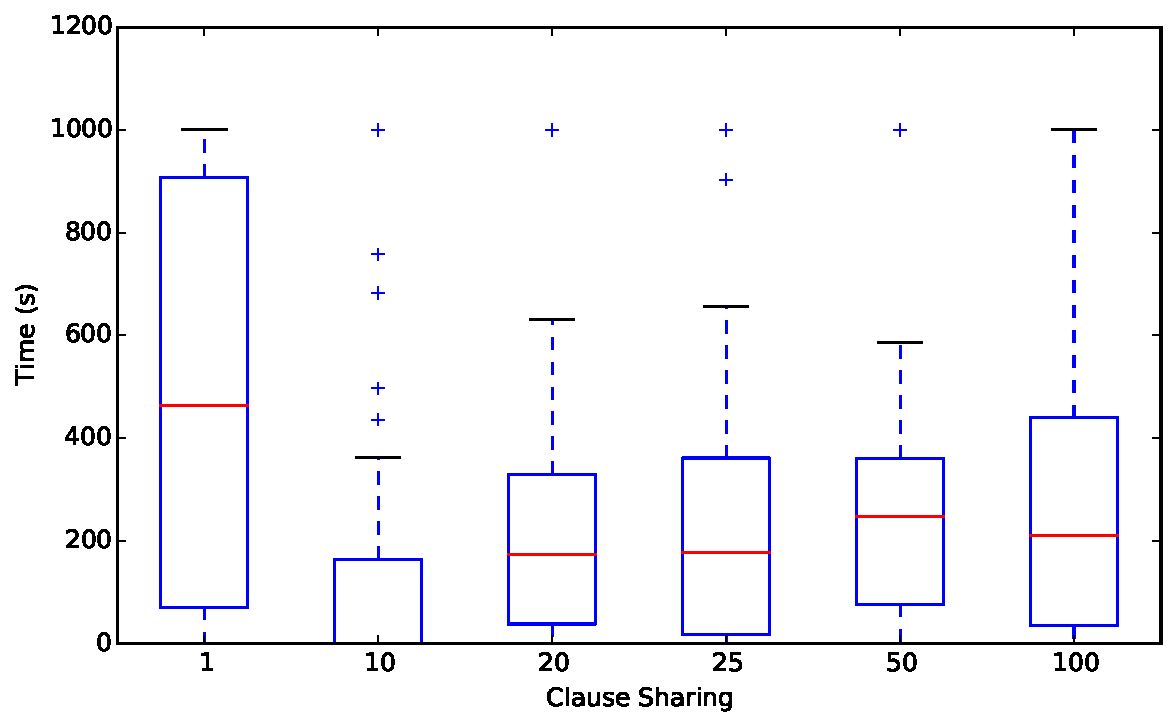
\includegraphics[width=0.8\textwidth]{../figs/boxplot_all.pdf}
  \caption{Summary of running times}
  \label{fig:boxplot-1}
\end{figure}

\subsection{ManySAT Results}


\section{Distributed ManySAT}
Details about the proposed implementation. 



\end{document}